% This file provides an example Beamer presentation using the RWTH theme
% showcasing some of the more common options, similar to the Powerpoint version
% 12.11.2014: Revision 1 (Harold Bruintjes, Tim Lange)

% For RWTH, beamer should be loaded with class option t (top)
\documentclass[t]{beamer}

% Use fontspec to get Arial font
% Requires use of XeLaTeX
\usepackage{fontspec}
\setmainfont{Arial}
\setsansfont{Arial}
% Also force Arial for math for a more consistent look
\usepackage{unicode-math}

% German style date formatting (footer)
\usepackage[ddmmyyyy]{datetime}
\renewcommand{\dateseparator}{.}

\usepackage{MnSymbol,wasysym}

% Format the captions used for figures etc.
\usepackage[compatibility=false]{caption}
\captionsetup{singlelinecheck=off,justification=raggedleft,labelformat=empty,labelsep=none}

% PGFPlots is used for drawing some of the charts
\usepackage{pgfplots}
\pgfplotsset{compat=newest}
% This file contains some styles and macros for drawing charts similar to those of MS Office

\pgfplotsset{hor_barchart/.style={
  xbar=0mm,
  xmin=0,
  xtick=\empty,
  axis y line*=left,
  x axis line style={opacity=0},
  bar width=0.6cm,
  ytick=data,
  nodes near coords,
  every axis/.append style={font=\normalsize},
  every node near coord/.append style={font=\normalsize},
  nodes near coords align={horizontal},
  legend style={at={(0,-10mm)},anchor=north west,legend columns=-1,draw=none},
}}

\pgfplotsset{ver_barchart/.style={
  ybar=0mm,
  x = 4.5cm,
  ymin=0,
  ymajorgrids,
  axis x line*=bottom,
  y axis line style={opacity=0},
  bar width=0.8cm,
  enlarge x limits={0.15},
  xtick=data,
  nodes near coords,
  every axis/.append style={font=\normalsize},
  every node near coord/.append style={font=\normalsize},
  nodes near coords align={vertical},
  legend style={at={(0,-10mm)},anchor=north west,legend columns=-1,draw=none},
}}

\tikzstyle{chart}=[
    legend label/.style={font={\normalsize},anchor=west,align=left},
    legend box/.style={rectangle, draw=none, minimum size=5pt},
]

\tikzstyle{pie chart}=[
    chart,
    slice/.style={line cap=round, line join=round,draw=none},
    pie title/.style={font={\bf}},
    slice type/.style 2 args={
        ##1/.style={fill=##2},
        values of ##1/.style={}
    }
]

\newcommand{\pie}[3][]{
    \begin{scope}[#1]
    \pgfmathsetmacro{\curA}{90}
    \pgfmathsetmacro{\r}{1}
    \def\c{(0,0)}
    \node[pie title] at (90:1.3) {#2};
    \foreach \v/\s in{#3}{
        \pgfmathsetmacro{\deltaA}{\v/100*360}
        \pgfmathsetmacro{\nextA}{\curA + \deltaA}
        \pgfmathsetmacro{\midA}{(\curA+\nextA)/2}

        \path[slice,\s] \c
            -- +(\curA:\r)
            arc (\curA:\nextA:\r)
            -- cycle;

        %\begin{pgfonlayer}{foreground}
        % Position labels at 1.2 times radius (just outside of chart)
        \path \c -- node[pos=1.2,pie values,values of \s]{$\v\%$} +(\midA:\r);
        %\end{pgfonlayer}

        \global\let\curA\nextA
    }
    \end{scope}
}

% Custom legend (used for pie chart)
\newcommand{\legend}[2][]{
\begin{scope}[#1]
  \path
    \foreach \n/\s in {#2} {
      ++(0,-5pt) node[\s,legend box] {} +(5pt,0) node[legend label] {\n}
    };
\end{scope}
}


%custom
\usepackage{tikz}
\usetikzlibrary{trees}
\usetikzlibrary{automata, positioning}
\usepackage{listings}
\lstset{basicstyle=\ttfamily}
\usepackage{tcolorbox}
\usepackage{framed}
\usepackage{forest}
\usepackage{xcolor}
\usepackage{blkarray}
\usepackage{comment}

%\usepackage{mathtools}
\renewcommand{\Coloneqq}{\mathrel{\mathop{::}}=}
\newcommand*{\mybox}[1]{\framebox{#1}}
\begin{comment}
    \definecolor{lightred}{RGB}{255,179,179}
    \definecolor{darkred}{RGB}{153,38,0}
    \definecolor{textred}{RGB}{255,77,77}

    \newenvironment{definitionblock}[1]{%
        \setbeamercolor{block body}{bg=lightred,fg=black}
        \setbeamercolor{block title}{bg=textred,fg=darkred}
        \begin{block}{#1}}{\end{block}}
\end{comment}


\setbeamertemplate{bibliography item}{\insertbiblabel}


%\setbeamertemplate{caption}[numbered]

% Load the actual RWTH theme. Suggested is to load the full theme,
% as it requires some specific dimensions
\usetheme{rwth}

\begin{document}

    \logo{
\includegraphics{logo.png}}

% Setup presentation information
    \title{Auflösen von Mehrdeutigkeiten in kontextfreien Grammatiken}
    \date{17.05.2024}
    \author{Lennart Protte}

    \frame{\titlepage}


    \section{Mehrdeutige Grammatik}\label{sec:mehrdeutige-grammatik2}
    \begin{frame}
        \vspace{-1em}
        \begin{columns}[T]
            \begin{column}{0.50\textwidth}
                \centering
                \begin{block}{Grammatik}
                    \vspace{-1em}
                    \begin{minipage}[t]{\linewidth}
                        \begin{align*}
                            & G(N,T,P,S) \\
                            & N= \{E\} \\
                            & T= \{+, *, \bold{num}\} \\
                            & S= \{E\}  \\
                            & P = \{ \\
                            & E \rightarrow E + E | E * E | \bold{num} \\
                            & \}
                        \end{align*}
                    \end{minipage}
                \end{block}
                \bigskip
                \begin{block}{Definition\cite{softwarelanguage}}
                    Eine Grammatik ist mehrdeutig, wenn sie mehrere Ableitungen für ein Wort zulässt.
                \end{block}
            \end{column}
            \begin{column}{0.33\textwidth}
                \centering
                \begin{block}{Ableitungen}
                    \vspace{-1em}
                    \begin{minipage}[t]{\linewidth}
                        \begin{align*}
                            & E \rightarrow E + E \\
                            & \phantom{E} \rightarrow E + E * E \\
                            & \phantom{E} \rightarrow \bold{num} + E * E \\
                            & \phantom{E} \rightarrow \bold{num} + \bold{num} * E \\
                            & \phantom{E} \rightarrow \bold{num} + \bold{num} * \bold{num} \\
                        \end{align*}
                        \vspace{-2em}
                        \begin{align*}
                            & E \rightarrow E + E \\
                            & \phantom{E} \rightarrow \bold{num} + E \\
                            & \phantom{E} \rightarrow \bold{num} + E * E \\
                            & \phantom{E} \rightarrow \bold{num} + \bold{num} * E \\
                            & \phantom{E} \rightarrow \bold{num} + \bold{num} * \bold{num} \\
                        \end{align*}
                    \end{minipage}
                \end{block}
            \end{column}
        \end{columns}
    \end{frame}


    \section{Definition der Chomsky-Normalform}\label{sec:chomsky-normal-form-definition}
    \begin{frame}
        \begin{block}{Definition\cite{watrous2020}}
            Eine kontextfreie Grammatik ist in der Chomsky-Normalform, wenn jede Produktionsregel eine der folgenden Formen hat:
            \begin{align*}
                & A \rightarrow BC \\
                & A \rightarrow a \\
                & S \rightarrow \varepsilon
            \end{align*}
            Hierbei sind $A,B,C \in N$, $S \in \text{Startsymbol}$ und $a \in T$. \\
            Für $B$ und $C$ gilt $B,C \neq S$.
        \end{block}
    \end{frame}


    \section{Chonsky Normal Form Beispiel}\label{sec:chonsky-normal-form-beispiel}
    %hier dann beispielhaften baum anzeichnen in präsentation
    \begin{frame}
        \centering
        \vspace{-1em}
        \begin{minipage}[c]{0.4\textwidth}
            \begin{block}{CFG}
                \vspace{-1em}
                \begin{align*}
                    & G(N,T,P,S) \\
                    & N= \{E\} \\
                    & T= \{+, *, \bold{num}\} \\
                    & S= \{E\}  \\
                    & P = \{ \\
                    & E \rightarrow E + E | E * E | \bold{num} \\
                    & \}
                \end{align*}
            \end{block}
        \end{minipage}%
        \quad%
        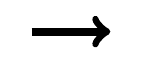
\begin{tikzpicture}
            \draw[->, line width=1mm](0,0) -- (1,0);
        \end{tikzpicture}%
        \quad%
        \begin{minipage}[c]{0.4\textwidth}%
            \begin{block}{CNF}
                \vspace{-1em}
                \begin{align*}
                    & G'(N,T,P,S) \\
                    & N= \{S, E, H_0, H_1, H_2, H_3\} \\
                    & T= \{+, *, \bold{num}\} \\
                    & S= \{S\}  \\
                    & P = \{ \\
                    & S \rightarrow H_0 E | H_1 E | \bold{num} \\
                    & E \rightarrow H_0 E | H_1 E | \bold{num} \\
                    & H_0 \rightarrow E H_2 \\
                    & H_1 \rightarrow E H_3 \\
                    & H_2 \rightarrow + \\
                    & H_3 \rightarrow * \\
                    & \}
                \end{align*}
            \end{block}
        \end{minipage}
    \end{frame}


    \section{Baum von $G'$}\label{sec:baum-von-$g'$}
    \begin{frame}
        \begin{block}{Beispielhafter AST von $G'$}
            \centering
            \begin{forest}
                [*
                [*
                [*
                [E]
                [E]
                ]
                [+
                [E]
                [E]
                ]
                ]
                [+
                [+
                [E]
                [E]
                ]
                [*
                [E]
                [E]
                ]
                ]
                ]
            \end{forest}
        \end{block}
        \bigskip
        \begin{exampleblock}{Bewerkung\cite{watrous2020}}
            Jeder, aus einer CNF erzeugter Baum, ist ein Binärbaum.
        \end{exampleblock}
    \end{frame}

    \section{Lösen von Mehrdeutigkeiten bei Operatoren}\label{sec:losen-von-merhdeutigkeiten-bei-operatoren}
    \begin{frame}
        \begin{block}{Probleme der Chomsky Normal Form}
            \begin{itemize}
                \item Keine Aussage über die Mehrdeutigkeit einer Grammatik
                \item Für komplexe Sprachen werden viele Produktionen benötigt
            \end{itemize}
        \end{block}
        \bigskip\bigskip
        \begin{block}{Methode zur Beseitigung von Mehrdeutigkeiten}
            \begin{itemize}
                \item Durch Operatorvorrang und Operatorassoziativität können alle Mehrdeutigkeiten beseitigt werden
                \item Die Grammatik kann weiterhin kontextfrei bleiben
            \end{itemize}
        \end{block}
    \end{frame}

    \section{Definition von Mustern}\label{sec:muster}
    \begin{frame}
        \begin{block}{Definition\cite{softwarelanguage}}
            \vspace{-1em}
            \begin{align*}
                &\text{Gegeben ist das Tupel } (S, \alpha \circ \beta, \gamma) \text{ mit:} \\
                &S \text{ = Das Startsymbol der Produktion} \\
                &\alpha \circ \beta \text{ = zwei Nichtterminale aus } G \text{ mit } \circ \text{ als Operator} \\
                &\gamma \text{ = Die Ableitung} \\
                &\text{Ob } \alpha \text{ oder } \beta \text{ abgeleitet wird,} \\
                &\text{wird durch ein } \bullet \text{ vor dem jeweiligen Nichtterminal gekennzeichnet.}
            \end{align*}
        \end{block}
        \bigskip
        \begin{exampleblock}{Beispiel}
            So kann $E \Rightarrow E + E \Rightarrow \mathbf{num} + E \Rightarrow \mathbf{num} + \mathbf{num}$ \\ durch
            $(E, \bullet{E}+E, \mathbf{num})$ und $(E, E+\bullet{E}, \mathbf{num})$ beschrieben werden.
        \end{exampleblock}
    \end{frame}


    \section{Tabellen für Ordnung und Assoziativität}\label{sec:tabellen-fur-ordnung-und-assotiativitat}
    \begin{frame}
        \begin{block}{Aus der Ordnung $ \alpha_{1} > \alpha_{2}$ ergibt sich:}
            \begin{table}[h]
                \centering
                \begin{tabular}{|c|c|}
                    \hline
                    >                          & $E \Coloneqq E\alpha_{2}E$                   \\
                    \hline
                    $E \Coloneqq E\alpha_{1}E$ & $(E, \bullet{E}\alpha_{1}E, {E}\alpha_{2}E)$ \\
                    & $(E, E\alpha_{1}\bullet{E}, E\alpha_{2}E)$   \\
                    \hline
                \end{tabular}\label{tab:table}
            \end{table}\cite{softwarelanguage}
        \end{block}
        \bigskip\bigskip
        \begin{block}{Aus $\alpha_{1}, \alpha_{2}$ sind links assoziativ folgt:}
            \begin{table}[h]
                \centering
                \begin{tabular}{|c|c|c|}
                    \hline
                    links                      & $E \Coloneqq E\alpha_{1}E$                 & $E \Coloneqq E\alpha_{2}E$                 \\
                    \hline
                    $E \Coloneqq E\alpha_{1}E$ & $(E, E\alpha_{1}\bullet{E}, E\alpha_{1}E)$ & $(E, E\alpha_{1}\bullet{E}, E\alpha_{2}E)$ \\
                    \hline
                    $E \Coloneqq E\alpha_{2}E$ & $(E, E\alpha_{2}\bullet{E}, E\alpha_{1}E)$ & $(E, E\alpha_{2}\bullet{E}, E\alpha_{2}E)$ \\
                    \hline
                \end{tabular}\label{tab:table2}
            \end{table}\cite{softwarelanguage}
        \end{block}
    \end{frame}


    \section{Beispiel Algorithmus}\label{sec:beispiel-algorithmus}
    \begin{frame}
        \centering
        \begin{block}{Definition der Grammatik:}
            \centering
            \[E \Coloneqq E * E \phantom{|} (links) > E + E (links) | \bold{num} \]
            \bigskip
            \begin{tabular}{|c|c|c|}
                \hline
                Operator & Vorrang & Assoziativität   \\
                \hline
                *        & 2       & links assoziativ \\
                \hline
                +        & 1       & links assoziativ \\
                \hline
            \end{tabular}\label{tab:table4}
        \end{block}
        \bigskip\bigskip
        \begin{exampleblock}{Beispiel}
            So wird $2 + 3 * 4$ gemäß der definierten Assoziativität und der Vorrangsregeln eindeutig als
            $2 + (3 * 4)$ ausgewertet, was korrekt ist.
        \end{exampleblock}
    \end{frame}

    \begin{frame}
        \vspace{-1em}
        \begin{columns}[T]
            \begin{column}{0.33\textwidth}
                \centering
                \begin{block}{Muster zur Beseitigung der Mehrdeutigkeit}
                    \begin{minipage}[t][7.5cm]{\linewidth}
                        \vspace{-1em}
                        \begin{align*}
                        (E, E*\bullet{E}, E*E)
                            \\
                            (E, \bullet{E}*E, E+E) \\
                            (E, E+\bullet{E}, E*E) \\
                            (E, \bullet{E}+E, E+E)
                        \end{align*}
                    \end{minipage}
                \end{block}
            \end{column}
            \begin{column}{0.45\textwidth}
                \centering
                \begin{block}{Nach der Erstellung von neuen Nichtterminalen}
                    \begin{minipage}[t]{\linewidth}
                        \vspace{-1em}
                        \begin{align*}
                            & G(N,T,P,S) \\
                            & N = \{E, E_1, E_2, E_3, E_4\} \\
                            & T = \{+, *, \bold{num}\} \\
                            & S = \{E\} \\
                            & P = \{ \begin{aligned}[t]
                                         \\
                                         E &\rightarrow E_1 * E_2 | E_3 + E_4 | \bold{num} \\
                            \end{aligned} \\
                            & \}
                        \end{align*}
                    \end{minipage}
                \end{block}
            \end{column}
        \end{columns}
    \end{frame}


    \begin{frame}
        \centering
        \begin{minipage}[c]{0.45\textwidth}
            \begin{block}{Nach der Erstellung von neuen Produktionsregeln}
                \vspace{-2em}
                \begin{align*}
                    & G(N,T,P,S) \\
                    & N= \{E, E_1, E_2, E_3, E_4\} \\
                    & T= \{+, *, \bold{num}\} \\
                    & S= \{E\} \\
                    & P = \{ \\
                    & E     \rightarrow E_1 * E_2 | E_3 + E_4 | \bold{num} \\
                    & E_1   \rightarrow E_1 * E_2 | \bold{num} \\
                    & E_2   \rightarrow E_3 + E_4 | \bold{num} \\
                    & E_3   \rightarrow E_1 * E_2 | \bold{num} \\
                    & E_4   \rightarrow E_3 + E_4 | \bold{num} \\
                    & \}
                \end{align*}
            \end{block}
        \end{minipage}%
        \quad\quad%
        \begin{minipage}[c]{0.45\textwidth}
            \vspace{-1em}
            \begin{exampleblock}{Beispiel aufgelöster Produktionsregel}
                Für beispielsweise $E + E + E$ gibt es nur noch eine Möglichkeit:
                \begin{align*}
                    & E \rightarrow E_3 + E_4 \\
                    & \phantom{E} \rightarrow E_3 + E_3 + E_4 \\
                \end{align*}
                Das Muster $(E, \bullet{E}+E, E+E)$ verhindert die Alternative.
            \end{exampleblock}
        \end{minipage}
    \end{frame}

    \begin{frame}
        \centering
        \begin{minipage}[c]{0.45\textwidth}
            \vspace{-1em}
            \centering
            \begin{block}{Nach dem Prüfen von verschachtelten Fällen}
                \vspace{-2em}
                \begin{align*}
                    & G(N,T,P,S) \\
                    & N= \{E, E_1, E_2, E_3, E_4, E_5\} \\
                    & T= \{+, *, \bold{num}\} \\
                    & S= \{E\} \\
                    & P = \{ \\
                    & E     \rightarrow E_1 * E_2 | E_3 + E_4 | \bold{num} \\
                    & E_1   \rightarrow E_1 * E_5 | \bold{num} \\
                    & E_2   \rightarrow E_3 + E_4 | \bold{num} \\
                    & E_3   \rightarrow E_5 * E_2 | \bold{num} \\
                    & E_4   \rightarrow E_3 + E_4 | \bold{num} \\
                    & E_5   \rightarrow \bold{num} \\
                    & \}
                \end{align*}
            \end{block}
        \end{minipage}%
        \quad\quad%
        \begin{minipage}[c]{0.45\textwidth}
            \vspace{-1em}
            \centering
            \begin{exampleblock}{Bemerkung}
                \begin{itemize}
                    \item Die Vorrangs und Assoziativitätsregeln sind in der Produktion umgesetzt.
                    \item Die Grammatik ist nun eindeutig.
                    \item Die Grammatik ist frei von Zyklen
                \end{itemize}
            \end{exampleblock}
        \end{minipage}
    \end{frame}


    \section{Quellen}\label{sec:quellen}
    \begin{frame}[allowframebreaks]
        \bibliographystyle{apalike}
        \bibliography{refs}
    \end{frame}

\end{document}
